\documentclass{template}
\usepackage{enumitem}

\newcommand{\version}{Version 1.1}
\author{Denis Ivan Blazevic, \url{denbl369@student.liu.se}\\
  Frans Bergström, \url{frabe808@student.liu.se}\\
    }
\title{Designspecifikation}
\date{2016-12-16}
\rhead{Denis Ivan Blazevic\\
Frans Bergström\\
}




\begin{document}
\projectpage

\tableofcontents
\newpage

\section{Revisionshistorik}
\begin{table}[!h]
\begin{tabularx}{\linewidth}{|l|X|l|}
\hline
Ver. & Revisionsbeskrivning & Datum \\\hline
1.2 & Andra versionen av designspecifikationen. & 161218 \\\hline
1.1 & Första versionen av designspecifikationen. & 161216 \\\hline
\end{tabularx}
\end{table}

\section{Beskrivning utav spelets uppbyggnad}
Vår design utav spelet bygger på en spelmotor som har kontroll över tre stycken scener. Dessa scener är uppdelade i MenuScene, GameScene och EndScene som alla ärver från en IScene klass. Scenerna skapas och lagras i en lista som håller koll på vad nästa scen kommer att vara om spelomgången avslutas. Scenerna i sig har en HandleEvent, Draw och Update funktion där vi loopar igenom alla objekten i scenerna och kallar på respektive funktion. Objekten ärver från sf::Sprite (SFML klass) och är i sig en behållare av komponenter och variablar/funktioner för position och vilken bild som ska ritas. Objektet anropar då komponenternas HandleEvent, Update funktion där själva logiken och datan för objekten hanteras.

I vår spelmotorn har vi valt att arbeta med komponentbaserade klasser, det gör att vi inte jobbar med direkta klass arv. Istället har vi skapat ett komponent system som hjälper oss att skapa många olika objekt med olika typer av komponenter tillhörandes. Till exempel kan vi skapa ett objekt som har komponenterna Moveable, PlayerComponent, Collision och PlayerController - och detta ger oss då en spelar klass. Anledningen till varför vi valde att göra på detta sätt var för att lära oss om komponentbaserad uppbyggnad av program och hur de kan vara till hjälp vid större projekt. Vi valde även att göra det på så vis för att vi ville kunna utveckla spelet vidare utan att behöva skriva om större delar av spelet - behövs ett nytt hinder i spelet så kan vi bara skapa ett nytt objekt som har helt andra komponenter som fungerar som ett hinder.

Det negativa med ett komponentbaserat system är dock att det är svårare att implmentera bra, då det är ännu viktigare att komponenterna fyller ett speciellt syfte. Vår design var när det gällde spelare var att PlayerController tar hand om input från spelaren, medan PlayerComponent användes för att spara och hantera variabler såsom kaffe och logik för om spelaren hoppar eller inte. Vi hade kunnat göra det ännu mer uppdelat att t.ex skapa en egen komponent för Coffee och Jump, dock med tanke på projektets storlek kändes det onödigt. Vi hade kunnat förbättra vårt komponentsystem ännu mer genom att dela upp logiken och data så att komponenterna bara har data medan olika system hanterar logiken. Detta hade ökat flexibiliteten och ökat prestandan på grund av t.ex mindre funktionsanropp. Dock är detta väldigt svårt att implementera och hade troligen behövt vara sin egna uppgift. En stor majoritet av vår tid spenderades på att få ihop komponentsystemet att fungera korrekt och därför fick vi inte mycket tid till att fina upp och utveckla själva spelet. Därför om vårt mål var att få så många funktioner som möjligt till spelet på så kort tid hade en mer klassiskt hierarkimodell varit smidigare, men mindre modulärt om vi vill ändra något.

\subsection{Klassdiagram}
Nedan kommmer en nedskalad bild av klassdiagrammet. Bilden finns även externt och kan därför användas till mer detaljerad visning. \\
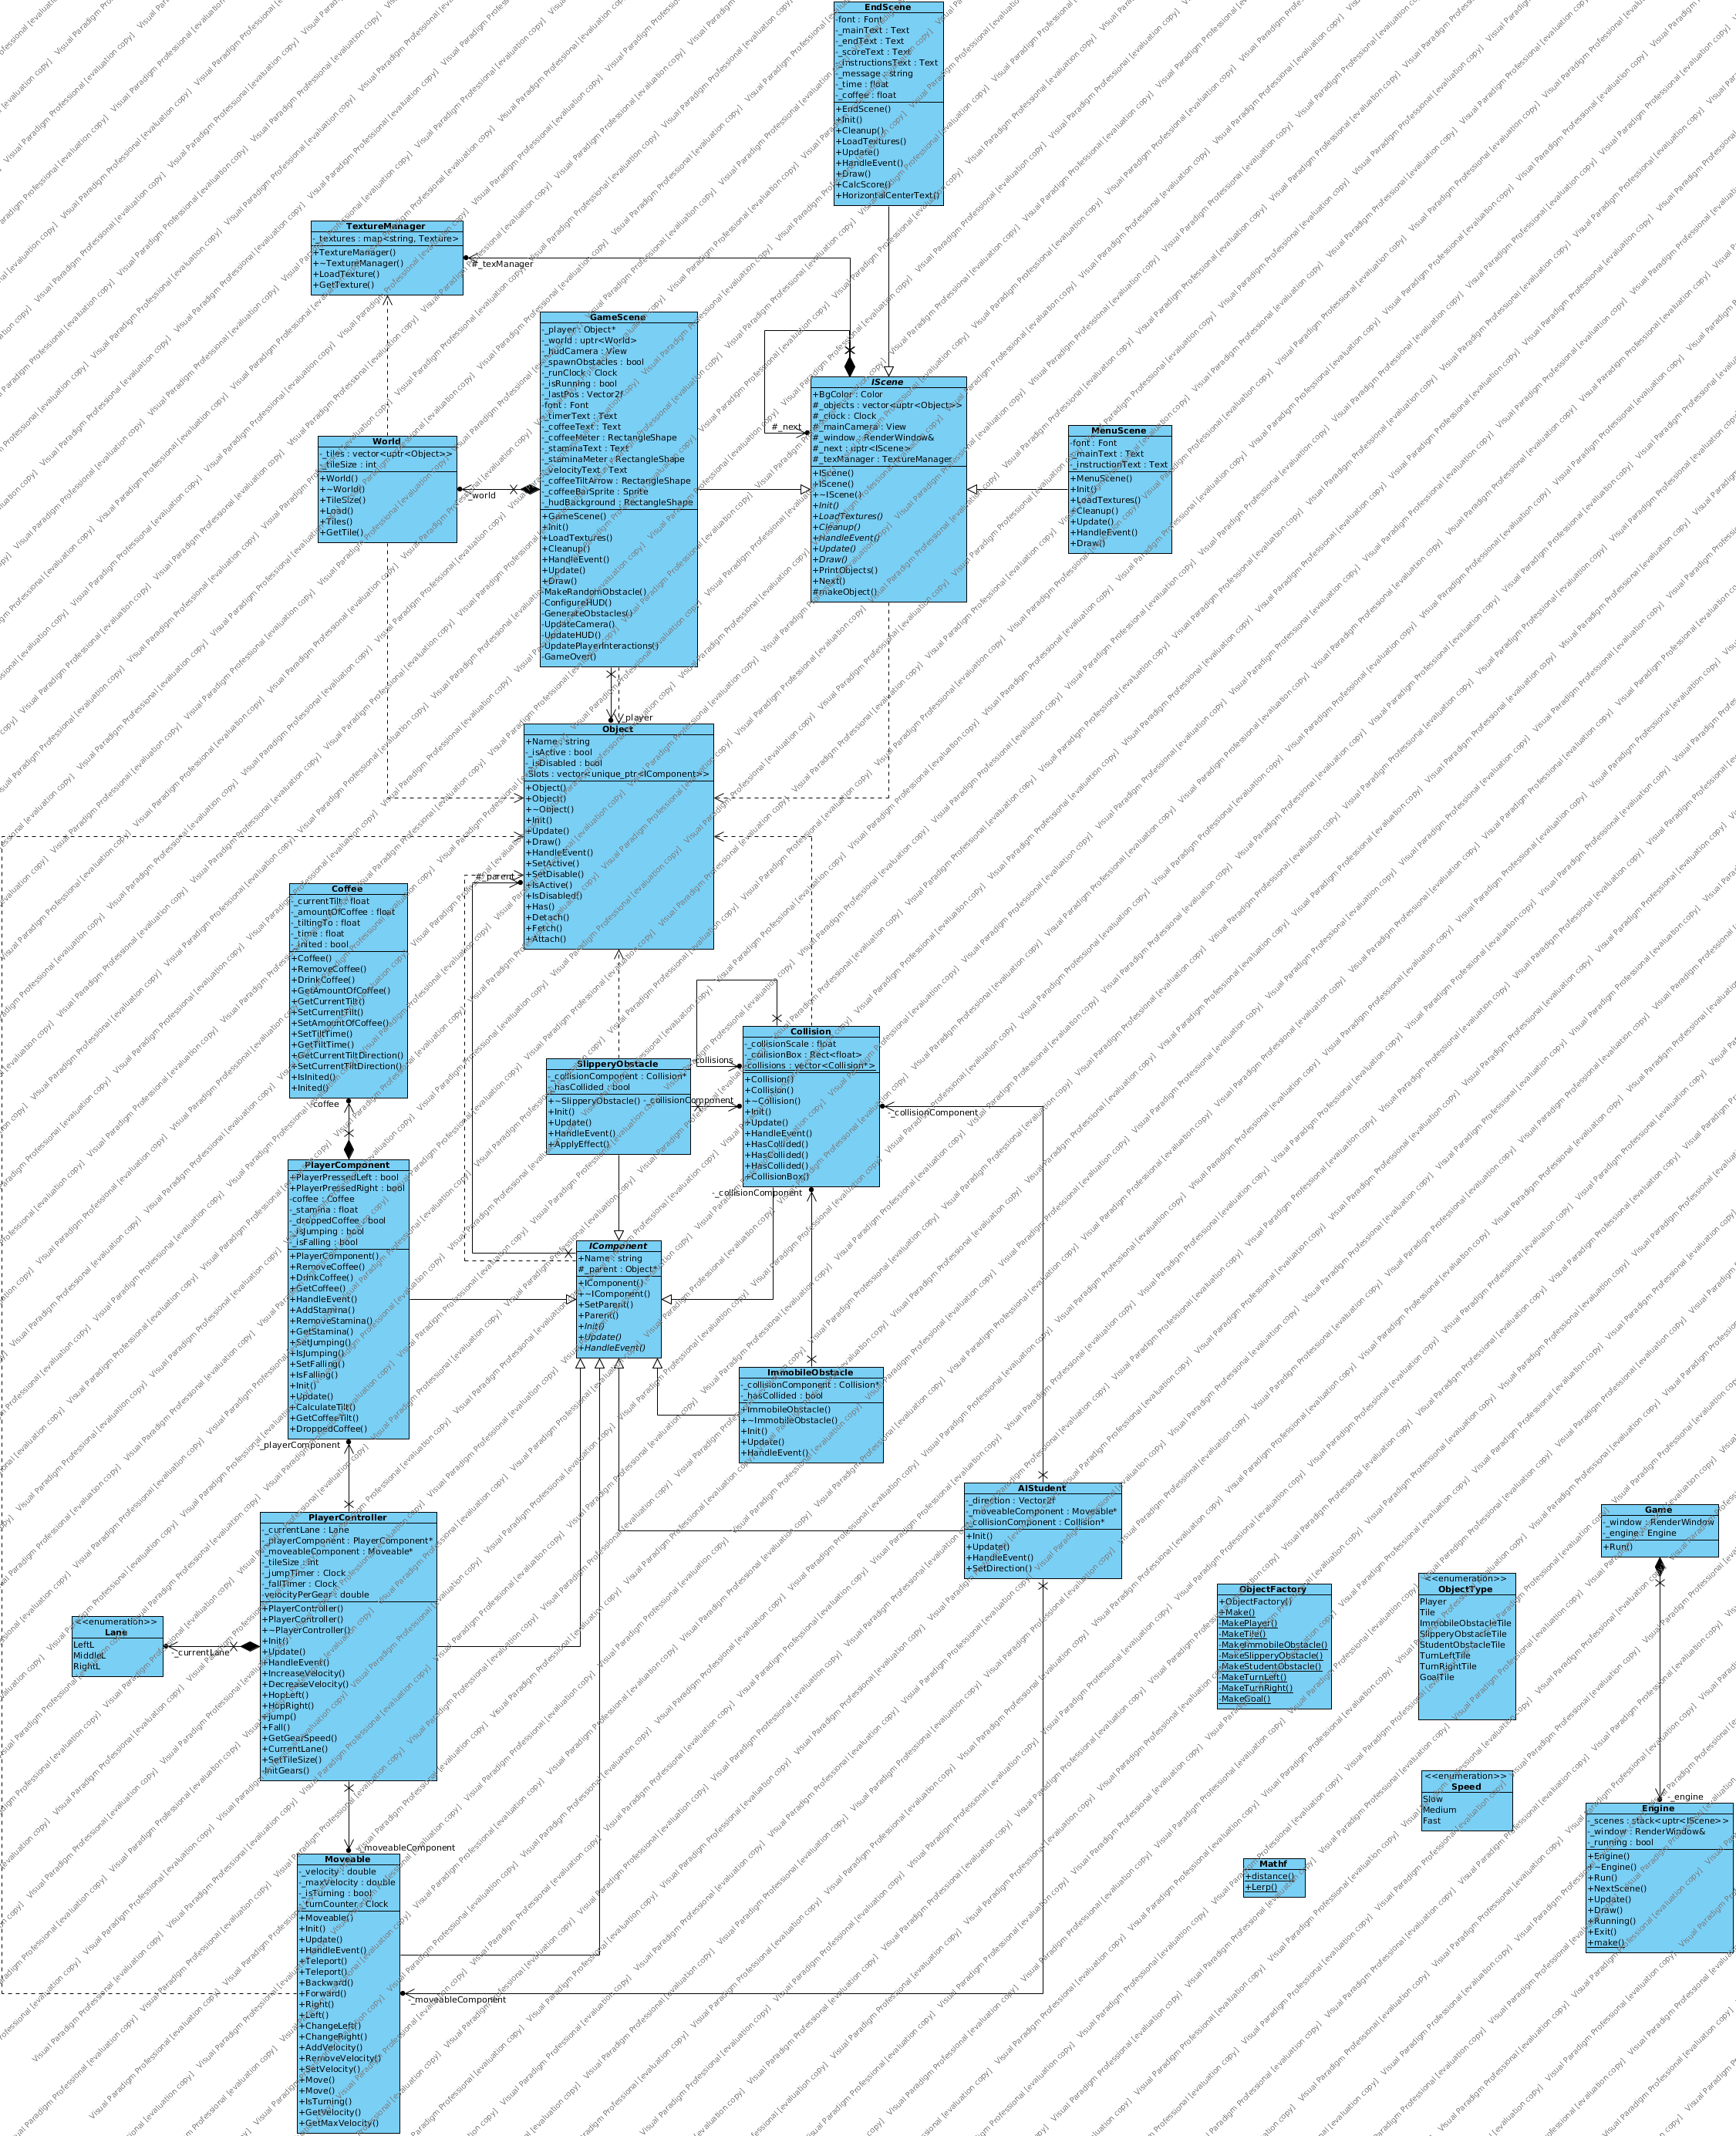
\includegraphics[width=40em]{klassdiagram1.png}
\newpage

\section{Detaljbeskrivning av Collision-klassen}
Collision-klassen ärver utav IComponent och agerar då som en komponent som implementeras till varje objekt där kollision önskas.Eftersom den ärver från IComponent har den tre abstrakta funktioner som måste överskrivas; Init, HandleEvents och Update. Övriga funktioner och variablar som finns är:

\begin{itemize}
\item Object * HasCollided() - Om ägaren av komponenten kolliderar med ett annat objekt som har en kollision komponent, returnera en pekare till det objektet. Loopar igenom den statiska listan och kontrollerar CollisionBox för varje Collision. 

\item Object * HasCollided(sf::Vector2) - Samma som ovan fast med en offset i form av en sf::Vector2f.

\item Object * HasCollided(float,float) - Samma som ovan fast med en offset i form av två floats för x och y-led.

\item sf::Rect<float> CollisionBox() - Returnerar collisionBox.

\item static std::vector<Collision *> collisions - En statisk lista av alla kollisions komponenter som finns i spelet.

\item float collisionScale - En faktor som används för att ändra boxens storlek förhållande till objektets sprite. Standard är värde 1.

\item sf::Rect<float> collisionBox - Kollisions boxen som används vid kollisionhantering. Det uppdateras i update till att va samma som objektets getGlobalBounds() (vilket ärvs från sf::Sprite) men kan ändra beroende på collisionScale.
\end{itemize}

{\setlength{\parindent}{0cm}
Konstruktorna och desktrukorn är följande:
}

\begin{verbatim}
Collision ()
Collision (float collisionScale)
~Collision ()
\end{verbatim}
Konstruktorn kommer lägga till sig själv i den statiska listan collisions så att alla Collision klasser har information om alla Collisions. I den andra konstruktorn kan man skicka in en collisionScale variabel som ändrar på collisionScale i klassen. Har den värde 0.5 kommer kollisionboxen vara hälften så stor som spriten som ritas ut. Destruktorn kommer sedan ta bort sin pekare från listan så de andra Collision klasserna inte längre kontrollerar kollision med döda objekt.

\newpage
\section{Detaljbeskrivning av World-klassen}
Syftet med World klassen är att kunna ladda in en map från en CSV (Comma-separated values) fil. Denna filen kommer sedan att loopas igenom och beroende på vad för nummer som finns har vi hårdkodat det till att respresentera ett speciellt objekt. T.ex kan 0 betyda att ett Floor objekt ska ritas där. Vi ökar också två variablar y och x för dess respektive loop för att få rätt position när vi skapar objektet. Vi definerar varje ökning i x-led för varje komma medan ökning i y sker vid radbryte. Objektet kommer sedan läggas i en lista där vi i World's Draw funktion ritar ut alla objekten. Andra funktioner och variablar som finns är:
\begin{itemize}
\item void Load(string filename, TextureManager) - Laddar in en CSV map och lägger in objekt i en lista med rätt position. Vilket objekt är hårdkortat för varje siffra i CSV mappen. TextureManager är en klass som har kolla på alla Textures i spelet. World använder den för att lägga till rätt texture till de objekt som skapas.
\item std::vector<std::unique pointer<Object>> Tiles() - En referens till listan med alla tiles (objekt) som världen är uppbygd på.
\item Object * GetTile(double, double) - Returnerar om det finns ett objekt i World på kordinaterna som skickas in.
\item std::vector<std::unique pointer<Object>> tiles - Listan med alla tiles(objekt) som ritas ut. 
\item int tileSize - Storleken på objekten. Används främst utav andra klasser för att t.ex gå ett objekt bakåt osv.
\item const int TileSize() const - Get funktion för tileSize.
\end{itemize}

{\setlength{\parindent}{0cm}
Konstruktorna och desktrukorn är följande:
}

\begin{verbatim}
World ()
~World ()
\end{verbatim}
Konstruktorn och destrukorn fyller ingen speciell funktion, då de är helt tomma. Listan med object behöver ej avallokeras då det är unique pointers.

\newpage
\section{Externa filformat}
Vi använder oss bara utav ett filformat som vi kalalr CSV (Comma-separated values
). Det är som det låter bara en text-fil som har värden separerade med kommas. Fungerar som en extern lista. Det negativa är att vi måste hårdkoda vilka objekt som ska ritas ut eftersom själva CSV filen inte har någon information exakt vad som ska ritas bara ett nummer. 



\end{document}
